\section{Simulation Farming}\label{sec:farming}
\index{Doob-Gillespie algorithm!simulation farming}\index{farming!simulation}

%\textbf{Instructional Time:} 6 hours

A single trajectory reveals one possible outcome. Only a large sample reveals the distribution of outcomes and answers probabilistic questions such as ``what fraction of populations go extinct?'' We therefore run many simulations and aggregate their results.

We bring our results on Examples~\ref{ex:saline_tank}, \ref{ex:logistic_growth}, \ref{ex:allee}, and \ref{ex:sir_first} together to design Doob-Gillespie implementations for those examples. Every model reuses the simulation core functions \RatesToPmf{}, \RateToDeltaTime{}, and \PmfToEventIndex{} of Figure~\ref{fig:dg_algorithm} and its \texttt{Python} template (Listing~\ref{lst:dg_algorithm_python_template}). Only two subroutines are bespoke to each model: \MakeRates{} and \MakeDeltaStates{}. For each model below we give just these two, in pseudocode and in \texttt{Python}. Each model in the companion code inlines the same loop, replacing the Step 5 total-rate check with an absorbing-state guard where one is convenient, and the SIR model has a vector state $(S, I, R)$ that \UpdateSirState{} updates componentwise.

We look at the saline tank model in Example~\ref{ex:saline_tank_code} (simulating Example~\ref{ex:saline_tank}),\index{model!saline tank} the logistic growth model in Example~\ref{ex:logistic_growth_code},\index{logistic growth} the Allee effect model in Example~\ref{ex:allee_code} (Example~\ref{ex:allee}),\index{Allee effect} and the SIR epidemiological model in Example~\ref{ex:sir_code} (Example~\ref{ex:sir_first}),\index{model!SIR} in order of increasing model complexity.



\begin{example}\label{ex:saline_tank_code}
\textbf{Saline Tank DG Simulation.}
Reconsider Example~\ref{ex:saline_tank}. We implement the Doob-Gillespie algorithm and simulate $100,000$ trajectories with run times $T = 1000$ hours each. We estimate the probability that too many NaCl molecules enter the tank with the sample proportion\index{proportion, sample} of simulations in which the system state exceeded the tolerance.

We assume the tank has $V = 10^6$ liters, $a = b = 100$ liters per hour, $c = 2.9112 \times 10^{-26}$ grams per liter, and that one NaCl molecule has mass $m = 9.704 \times 10^{-23}$ grams. All simulations begin with $300$ NaCl molecules in the tank, and if the tank holds $310$ NaCl molecules at any time during a simulation, then the manufacturing process has failed.

This system with these parameters is a linear system with globally stable equilibrium $M = \frac{bcV}{m(a+b)} \approx 150$. Trajectories below $M = 150$ drift stochastically upward, while trajectories above $M = 150$ drift stochastically downward. Hence, even though our simulations start with $300$ molecules and the tolerance is $310$, fewer than half of all simulations should fail manufacturing tolerances.

Whenever $M > 0$, the event in which a salt molecule leaves the tank occurs with positive probability. A positive probability always exists that $M$ crashes to zero. We call such an occurrence \textit{stochastic extinction}.\index{extinction!stochastic} In this example, stochastic extinction is a temporary condition, because when $M = 0$, the next event must be an arrival and occurs with rate $\frac{bc}{m}$.

Table~\ref{tab:saline_tank_events} lists the two events.

\begin{table}[htbp]
\centering
\caption{Saline tank Doob-Gillespie events.}\label{tab:saline_tank_events}
\begin{tabular}{llll}
\hline
Event & Description & Rate & $\Delta$State \\
\hline
Arrival & Salt molecule enters tank & $\frac{bc}{m}$ & $+1$ \\
Departure & Salt molecule leaves tank & $\frac{(a+b)M}{V}$ & $-1$ \\
\hline
\end{tabular}
\end{table}

We emphasize that every model uses only two bespoke subroutines, \MakeRates and \MakeDeltaStates.
All the other functions in Figure~\ref{fig:dg_subroutines_a} and Figure~\ref{fig:dg_subroutines_b} are identical for all models.
Moreover, a simple lookup could replace the function \MakeDeltaStates rather than an explicit function, ostensibly simplifying our presentation of each model, but at the cost of complicating our template in Figure~\ref{fig:dg_algorithm} and Listing~\ref{lst:dg_algorithm_python_template}.

In Figure~\ref{fig:bespoke_saline_tank}, $\textsf{MakeRates}$ returns the two rates of Table~\ref{tab:saline_tank_events}, the arrival rate $bc/m$ and the departure rate $(a+b)M/V$, and $\textsf{MakeDeltaStates}$ returns the state-change vector $(+1, -1)$, the $+1$ for an arrival (index $0$) and the $-1$ for a departure (index $1$). The generic loop of Figure~\ref{fig:dg_algorithm} uses them unchanged. Listing~\ref{lst:framework_saline_tank} gives the \texttt{Python} implementation, which lists the parameters $a, b, c, V, m$ explicitly.

\begin{figure}[htbp]
\centering
{\footnotesize
\adjustbox{valign=t}{\fbox{\procedure{$\textsf{MakeRates}(M,\, \theta) \to \vec{\lambda}$:}{
\pcind \pcreturn \left(bc/m,\; (a+b)M/V\right)
}}}\qquad
\adjustbox{valign=t}{\fbox{\procedure{$\textsf{MakeDeltaStates}(\theta) \to (\delta_j)_{j=1}^{N}$:}{
\pcind \pcreturn (+1,\, -1)
}}}\par}
\caption{The two bespoke subroutines for the saline tank model. $\textsf{MakeRates}$ returns the arrival and departure rates, and $\textsf{MakeDeltaStates}$ returns the $\pm 1$ state changes, both following Table~\ref{tab:saline_tank_events}. The generic loop of Figure~\ref{fig:dg_algorithm} uses them. Compare to the \texttt{Python} in Listing~\ref{lst:framework_saline_tank}.}
\label{fig:bespoke_saline_tank}
\end{figure}

\lstinputlisting[float=htbp, language=Python, numbers=none, linerange={17-24}, caption={The bespoke \texttt{Python} functions for the saline tank model, \MakeTankRates{} and \MakeTankDeltaStates{}. We pair these with the pseudocode of Figure~\ref{fig:bespoke_saline_tank}.}, label={lst:framework_saline_tank}]{../simulation_frameworks/saline_tank.py}

A typical execution sees a few dozen simulations out of $100,000$ exceed tolerances, providing a sample proportion on the order of $10^{-4}$. See Figure~\ref{fig:saline_tank} for a typical simulation result: trajectories starting above the equilibrium $M \approx 150$ drift downward, matching the ODE analysis. See Section~\ref{subsec:plotting_utilities} for the trajectory-plotting code.

\begin{figure}[htbp]
\centering
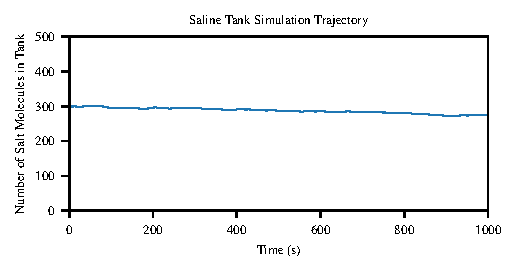
\includegraphics[width=\textwidth]{figures/saline_tank.pdf}
\caption{An example simulation from the model of Example~\ref{ex:saline_tank} with initial
condition $M(0) = 300 \textup{ NaCl molecules}$, parameters $V = 10^6\textup{ liters}$,
$a = b = 100\textup{ liters per hour}$,
$c=2.9112 \times 10^{-26}\textup{ grams per liter}$, assuming that one NaCl molecule has
mass $m = 9.704 \times 10^{-23}\textup{ grams}$, and with runtime $T=10^3\textup{ hours}$. We draw this with \PlotTrajs{} from \texttt{tools/plots/plot\_trajectories.py} (Listing~\ref{lst:plots_trajectories}).}
\label{fig:saline_tank}
\end{figure}

\end{example}


\begin{example}\label{ex:logistic_growth_code}
\textbf{Logistic Growth DG Simulation.}
Reconsider Example~\ref{ex:logistic_growth}, the logistic growth model. It is the simplest of our models: the state $P$ is a single population count changed by exactly two events. A birth increases $P$ by one and occurs at rate $rP$, and a death decreases $P$ by one and occurs at rate $rP^2/K$, where $r$ is the per-capita birth rate and $K$ is the carrying capacity. Table~\ref{tab:ode_events} lists the two events.

We simulate with a base doubling time $\tau = 36.5$ days, so that $r = \ln(2)/\tau$, a carrying capacity $K = 200$, an initial population $P(0) = 20$, and a run time $T = 365$ days.

In Figure~\ref{fig:bespoke_logistic_growth}, $\textsf{MakeRates}$ returns the birth rate $rP$ and the death rate $rP^2/K$ of Table~\ref{tab:ode_events}, and $\textsf{MakeDeltaStates}$ returns the state-change vector $(+1, -1)$, the $+1$ for a birth and the $-1$ for a death. Listing~\ref{lst:framework_logistic_growth} gives the \texttt{Python} implementation. It diverges from the pseudocode in deriving the per-capita rate $r = \ln(2)/\tau$ from the base doubling time, rather than taking $r$ directly.

\begin{figure}[htbp]
\centering
{\footnotesize
\adjustbox{valign=t}{\fbox{\procedure{$\textsf{MakeRates}(P,\, \theta) \to \vec{\lambda}$:}{
\pcind \pcreturn \left(rP,\; rP^2/K\right)
}}}\qquad
\adjustbox{valign=t}{\fbox{\procedure{$\textsf{MakeDeltaStates}(\theta) \to (\delta_j)_{j=1}^{N}$:}{
\pcind \pcreturn (+1,\, -1)
}}}\par}
\caption{The two bespoke subroutines for the logistic growth model. $\textsf{MakeRates}$ returns the birth and death rates, and $\textsf{MakeDeltaStates}$ returns the $\pm 1$ state changes, both following Table~\ref{tab:ode_events}. Compare to the \texttt{Python} in Listing~\ref{lst:framework_logistic_growth}.}
\label{fig:bespoke_logistic_growth}
\end{figure}

\lstinputlisting[float=htbp, language=Python, numbers=none, linerange={29-37}, caption={The bespoke \texttt{Python} functions for the logistic growth model, \MakeLogisticRates{} and \MakeLogisticDeltaStates{}. We pair these with the pseudocode of Figure~\ref{fig:bespoke_logistic_growth}.}, label={lst:framework_logistic_growth}]{../simulation_frameworks/logistic_growth.py}

The stochastic trajectories fluctuate around the deterministic logistic solution. Figure~\ref{fig:logistic_growth_mean_vs_ode} compares the mean of $30$ stochastic trajectories against the solution of Equation~\ref{eqn:logistic_growth}.

\end{example}


\begin{example}\label{ex:allee_code}
\textbf{Allee Effect DG Simulation.}
Reconsider Example~\ref{ex:allee} and the emperor's goal to estimate the probability that a colony goes extinct. We simulate trajectories with run times $T=2000$ days each and compute the sample proportion of simulations that go extinct. We assume the species has a base birth rate\index{birth rate} $r = 0.0045\textup{ days}^{-1}$, a cooperation threshold $L = 50\textup{ individuals}$, and a carrying capacity\index{carrying capacity} $K = 200\textup{ individuals}$. All colonies begin with $P(0) = 50$ individuals.

This system with these parameters has three equilibria. $P = 0$ and $P = K$ are stable equilibria, and $P = L$ is an unstable equilibrium. Trajectories with $0 < P < L$ or $P > K$ drift downward statistically. Trajectories with $L < P < K$ drift upward statistically. Since simulations start with $P(0) = 50 = L$, the first event is equally likely to be a birth or a death. About half of all trajectories will initially decrease and drift toward extinction. We therefore expect about half of all trajectories to end in extinction. Extinction is a permanent condition. Table~\ref{tab:allee_events} lists the four events.

\begin{table}[htbp]
\centering
\caption{Allee effect Doob-Gillespie events.}\label{tab:allee_events}
\begin{tabular}{llll}
\hline
Event & Description & Rate & $\Delta$State \\
\hline
Old-age death & Individual dies of old age & $\lambda_0 P$ & $-1$ \\
Sexual birth & Birth from sexual reproduction & $\lambda_0 P^2/K$ & $+1$ \\
Cooperative birth & Birth from cooperation & $\lambda_0 P^2/L$ & $+1$ \\
Competitive death & Death from over-competition & $\lambda_0 P^3/(KL)$ & $-1$ \\
\hline
\end{tabular}
\end{table}

In Figure~\ref{fig:bespoke_allee}, $\textsf{MakeRates}$ returns the four rates of Table~\ref{tab:allee_events} as the vector $(rP,\, rP^2/K,\, rP^2/L,\, rP^3/(KL))$, and $\textsf{MakeDeltaStates}$ returns the state-change vector $(-1, +1, +1, -1)$. Listing~\ref{lst:framework_allee} gives the \texttt{Python} implementation.

\begin{figure}[htbp]
\centering
{\footnotesize
\adjustbox{valign=t}{\fbox{\procedure{$\textsf{MakeRates}(P,\, \theta) \to \vec{\lambda}$:}{
\pcind \pcreturn \left(rP,\; \frac{r P^2}{K},\; \frac{r P^2}{L},\; \frac{r P^3}{KL}\right)
}}}\qquad
\adjustbox{valign=t}{\fbox{\procedure{$\textsf{MakeDeltaStates}(\theta) \to (\delta_j)_{j=1}^{N}$:}{
\pcind \pcreturn (-1,\, +1,\, +1,\, -1)
}}}\par}
\caption{The two bespoke subroutines for the Allee effect model, following Table~\ref{tab:allee_events}. Here $r$ is the base per-capita birth rate. Compare to the \texttt{Python} in Listing~\ref{lst:framework_allee}.}
\label{fig:bespoke_allee}
\end{figure}

The function \FindTraj{} (in the Python repository) inputs simulation setup data and a success condition function and returns a successful trajectory with a count of all attempts including the successful one. After running the Allee effect script (in the Python repository) with a sample of $128$ simulations, we saw $71$ simulations go extinct, providing an estimated probability of extinction $\widehat{p} = 0.5546875$ (see Section~\ref{subsec:background} for the definition of sample proportion and hat notation).
Verify that the qualitative behavior matches your ODE analysis: trajectories starting below $P = L = 50$ should drift toward extinction, while those starting above $L$ should drift toward $K = 200$.

\lstinputlisting[float=htbp, language=Python, numbers=none, linerange={9-19}, caption={\texttt{Python} functions \MakeAlleeRates{} and \MakeAlleeDeltaStates{} for the Allee effect model. See pseudocode in Figure~\ref{fig:bespoke_allee}.}, label={lst:framework_allee}]{../simulation_frameworks/allee_effect.py}

\begin{figure}[htbp]
\centering
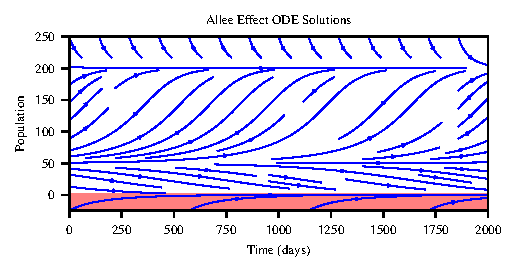
\includegraphics[width=\textwidth]{figures/allee_ode.pdf}
\caption{Phase diagram for Allee effect ODE $\frac{dP}{dt} = -rP(1-P/L)(1-P/K)$ ()$r = 0.0045\,\text{days}^{-1}$, $L = 50$, $K = 200$, from Example~\ref{ex:allee}).
Trajectories below $P = L$ trend to extinction. Trajectories above $P = L$ trend to $P = K$.
We shade the non-physical region $P < 0$ red. We draw this with \MakePhaseDiagram{} from \texttt{tools/plots/plot\_vector\_field.py} (Listing~\ref{lst:plots_vector_field}).}
\label{fig:allee_ode}
\end{figure}

\begin{figure}[htbp]
\centering
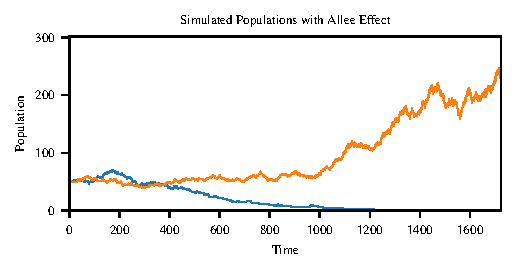
\includegraphics[width=\textwidth]{figures/allee_effect_two_trajs.pdf}
\caption{Two Allee trajectories from
Example~\ref{ex:allee}, with $r = 0.0045 (\text{time})^{-1}$,
$L = 50 \text{individuals}$, $K = 200$, and  $P(0) = 50$.  We draw this with \PlotTrajs{} from \texttt{tools/plots/plot\_trajectories.py} (Listing~\ref{lst:plots_trajectories}).}
\label{fig:allee_two_trajs}
\end{figure}


\begin{figure}[htbp]
\centering
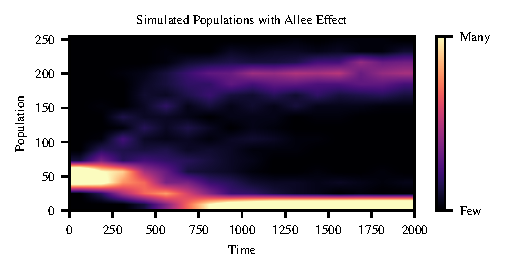
\includegraphics[width=\textwidth]{figures/allee_effect.pdf}
\caption{Heat map of $128$ Allee trajectories from Example~\ref{ex:allee} with the same parameters as Figure \ref{fig:allee_two_trajs}. Brighter pixels are near more trajectories.
We draw this with \PlotHeatmap{} from \texttt{tools/plots/plot\_heatmap\_histogram.py} (Listing~\ref{lst:plots_heatmap}).}
\label{fig:allee_heat}
\end{figure}

There are two types of stochastic trajectory. \textit{Successful} trajectories drift above $P(t) = L$ and reach the carrying capacity $P(t) = K$. \textit{Unsuccessful} trajectories slip below $P(t) = L$ and decline to extinction.
We use \PlotExtinctionAndSurvival{} to find two such trajectories in Figure~\ref{fig:allee_two_trajs}. See Section~\ref{subsec:plotting_utilities} for the plotting code.
The underlying ODE is scalar. We can therefore draw its phase diagram (Figure~\ref{fig:allee_ode}) as a streamplot in the $(t, P)$ plane. The streamlines confirm the three equilibria $P \in \{0, L, K\}$: trajectories starting below $L = 50$ converge to extinction, while those starting between $L$ and $K$ converge to the carrying capacity.
We generate a heat map of $128$ stochastic trajectories of the Allee model in Figure~\ref{fig:allee_heat}.
Nearly all trajectories fall into one of these two categories.
The heat map in Figure~\ref{fig:allee_heat} shows a proportion of simulations sweeping upward to the stable carrying capacity $P=K=200$, as well as a proportion falling below $P=L=50$ and ending near or at extinction.
The bright horizontal band around $P = 0$ at the end of the simulation indicates that many trajectories end in extinction.
The horizontal smear of brightness around $P = K = 200$ at the end of the simulation indicates that some trajectories survive at carrying capacity.
The darkness everywhere else indicate that trajectories don't spend a lot of time in the intermediate regions.
Hence, the distribution of simulation results at the end of the simulation is bimodal,\index{distribution!bimodal} with a cluster around $P = 0$ and a cluster around $P = K$.

As an aside, the state $P = 0$ is an absorbing state, so every window containing $P = 0$ contains many trajectories by the end of the simulation.
Thus, $P = 0$ appears very bright. In fact, in our Python code, we had to cap brightness to ensure that multimodal distributions would be visible.
The state $P = K$ is only probabilistically attracting, showing brightness in a haze around it, but trajectories wander nearby, dissipating their heat.
To make this graph, the heat map routine resamples every trajectory onto a common uniform time grid and then performs simple histogram binning.
That is to say, the heat indicates the residence of nearby trajectories, not the absolute number of nearby change-points.
See Section~\ref{subsec:plotting_utilities} for the heat-map plotting code and Section~\ref{subsubsec:prep_heatmap} for an explanation of this resampling.



The simulations are stochastic. Exceptions occur occasionally: trajectories bound for extinction that randomly wander above $P=L$ and recover to $P=K$, or trajectories near $P=K$ that randomly wander below $P=L$.

\end{example}


\begin{example}\label{ex:sir_code}
\textbf{SIR DG Simulation.}
Reconsider Example~\ref{ex:sir_first} and Charlie's fungus-infected cats. The SIR model partitions a population into three compartments: susceptible ($S$), infectious ($I$), and recovered ($R$). Individuals move from $S$ to $I$ upon infection and from $I$ to $R$ upon recovery. Assume Charlie has $S + I + R = 100$ cats, assume $I(0) = 10$ of the cats start out sick, and assume the rest are susceptible. We assume that cats recover with a half-life $\tau = 45$ days and interact with each other in random pairs $1000$ times a day, so the time between a cat's interactions is $\tau_{\textup{int}} = 1/1000 = 0.001$ days, and each interaction has a probability $0.0001$ (that is, $0.01\%$) of an infection spreading.
We use $\widetilde{\alpha} = \frac{0.0001}{0.001} = 0.1\,\textup{days}^{-1}$, and since $S + I + R = N = 100$, the per-pair rate is $\alpha = \widetilde{\alpha}/N = \frac{0.0001}{0.001 \cdot 100} = 10^{-3}\,(\textup{individual}\cdot\textup{days})^{-1}$, matching \MakeSirRates{} in the companion code.

We re-parameterize in terms of daily interactions because transmissibility depends on both the infectious organism and social behavior. For example, the black-tailed prairie dog is sociable, and plague (\textit{Yersinia pestis}) infections transmit rapidly through their populations. By contrast, California ground squirrels (\textit{Otospermophilus beecheyi}) are less social in their burrowing behavior and tolerate plague better than black-tailed prairie dogs \cite{buhnerkempe2011transmission}.

Unlike the previous models, the SIR state is a vector $(S, I, R)$ rather than a scalar count. Table~\ref{tab:sir_dg_events} lists the two events and their vector state changes.

\begin{table}[htbp]
\centering
\caption{SIR Doob-Gillespie events.}\label{tab:sir_dg_events}
\begin{tabular}{llll}
\hline
Event & Description & Rate & $\Delta$State \\
\hline
Infection & Susceptible becomes infectious & $\alpha S I$ & $(-1,+1,0)$ \\
Recovery & Infectious individual recovers & $\beta I$ & $(0,-1,+1)$ \\
\hline
\end{tabular}
\end{table}

In Figure~\ref{fig:bespoke_sir}, $\textsf{MakeRates}$ returns the infection rate $\alpha S I$ and the recovery rate $\beta I$ of Table~\ref{tab:sir_dg_events}, and, because the state is the vector $(S, I, R)$, $\textsf{MakeDeltaStates}$ returns the two vector changes $(-1, +1, 0)$ for an infection and $(0, -1, +1)$ for a recovery. Listing~\ref{lst:framework_sir} gives the \texttt{Python} implementation. It diverges from the pseudocode in two language- and model-specific ways: it derives $\alpha$ from the interaction time and infection probability and $\beta = \ln(2)/\tau$ from the recovery half-life, rather than taking $\alpha$ and $\beta$ directly, and it adds the chosen state change componentwise in \UpdateSirState{}.

\begin{figure}[htbp]
\centering
{\footnotesize
\adjustbox{valign=t}{\fbox{\procedure{$\textsf{MakeRates}((S,I,R),\, \theta) \to \vec{\lambda}$:}{
\pcind \pcreturn \left(\alpha S I,\; \beta I\right)
}}}\qquad
\adjustbox{valign=t}{\fbox{\procedure{$\textsf{MakeDeltaStates}(\theta) \to (\delta_j)_{j=1}^{N}$:}{
\pcind \pcreturn \left((-1, +1, 0),\; (0, -1, +1)\right)
}}}\par}
\caption{The two bespoke subroutines for the SIR model, following Table~\ref{tab:sir_dg_events}. Here $\alpha$ is the transmission rate and $\beta$ the recovery rate. The state change $\delta_j$ is a vector. Compare to the \texttt{Python} in Listing~\ref{lst:framework_sir}.}
\label{fig:bespoke_sir}
\end{figure}

\lstinputlisting[float=htbp, language=Python, numbers=none, linerange={13-29}, caption={The bespoke \texttt{Python} functions for the SIR model: \MakeSirRates{}, \MakeSirDeltaStates{}, and the componentwise update \UpdateSirState{}. We pair these with the pseudocode of Figure~\ref{fig:bespoke_sir}.}, label={lst:framework_sir}]{../simulation_frameworks/epidemiology.py}

We generate $100,000$ stochastic trajectories with run time $T = 365$ days (see the Python repository for the code) to estimate (i) the probability that Charlie's cats totally recover within a year and (ii) the five-number summary\index{summary, five-number} of the time until Charlie has no more infected cats, computed from trajectories in which all infectious cats recovered (i.e., $I = 0$) before day $365$. Our simulation reveals an estimated probability of total recovery within the year of $0.53844$ (a sample proportion, defined in Section~\ref{subsec:background}). The five-number summary (see Section~\ref{subsec:background}) of the time until recovery, computed only from trajectories in which all infectious cats recovered before day $365$, was $(161.5, 288.1, 315.9, 340.0, 364.998)$. This indicates that, when Charlie's cats totally recover within one year, a $50\%$ probability exists that the cats will take more than $316$ days to recover. We use the SIR plotting code (in the Python repository) to visualize one representative stochastic trajectory (which includes all three compartments of population members) in Figure~\ref{fig:sir}.

\begin{figure}[htbp]
\centering
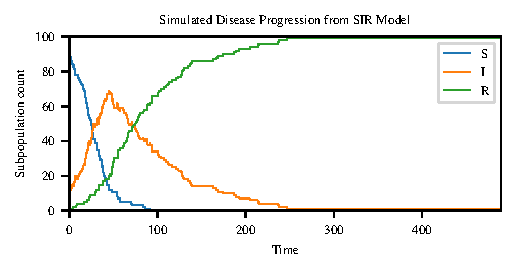
\includegraphics[width=\textwidth]{figures/epidemiology.pdf}
\caption{An example simulation of the fungal infection among Charlie's cats, showing the susceptible ($S$), infectious ($I$), and recovered ($R$) compartments over time. We draw this with \PlotTrajs{} from \texttt{tools/plots/plot\_trajectories.py} (Listing~\ref{lst:plots_trajectories}).}
\label{fig:sir}
\end{figure}

Verify that the qualitative behavior matches your ODE analysis: the susceptible compartment should fall monotonically, and the infectious compartment should peak and then decline as recovery outpaces new infections.

A streamplot like Figure~\ref{fig:ode_examples} does not apply here. A streamplot in the $(t, x)$ plane depicts the vector field $(1, f(t,x))$ for a scalar ODE $\dot{x} = f(t,x)$. The SIR state is the vector $(S, I, R)$ with conservation law $S + I + R = N$. The individual rates $\frac{dS}{dt} = -\alpha SI$ and $\frac{dI}{dt} = \alpha SI - \beta I$ each depend on two compartments. A phase portrait in the $(S, I)$ plane is possible, but it discards the time axis and does not give the timescale of the outbreak.

\end{example}




The examples above used sample proportions and five-number summaries to summarize simulation output. Section~\ref{subsec:background} introduces both. Section~\ref{subsec:output} formalizes their use, discusses when summary statistics can be misleading (particularly for bimodal output), and provides practical guidance for reporting stochastic simulation results. Read Section~\ref{subsec:output} before proceeding to sensitivity analysis (Section~\ref{subsec:qualitative_changes}), as the sensitivity analysis in Section~\ref{subsec:qualitative_changes} relies on the same statistical vocabulary.

\textup{{\bf Questions for Reflection:}}
\begin{enumerate}

\item Given $r, s > 0$ and the same initial condition $X_0 = Y_0$, the ODEs $\frac{dX}{dt} = rX$ and $\frac{dY}{dt} = (r+s)Y - sY$ always produce the same trajectories. Can you use the Doob-Gillespie algorithm to detect a difference between them? Explain.

\item In the deterministic Allee ODE, what happens as $L$ approaches $K$?

\item What can we expect from stochastic realizations of the Allee ODE as $L$ approaches $K$?

\item In the deterministic Allee ODE, what happens as we vary $r$?

\item What are some changes we can expect from the stochastic realizations of the Allee ODE as we vary $r$?

\item Consider the Allee-like model $\frac{dY}{dt} = rY(1-\frac{Y}{K})(1-\frac{Y}{L})(1-\frac{Y}{U})$ for some $K > L > U > 0$. Is this model suitable for describing a realistic ecological population with finite resources? Hint: Find the equilibria and determine whether birth or death is more likely near those equilibria.

\item How does your answer to the previous question change if we use $\frac{dY}{dt} = -rY(1-\frac{Y}{K})(1-\frac{Y}{L})(1-\frac{Y}{U})$ with the same $K > L > U > 0$? Hint: The sign change reverses time.

\item Interpret the notion of stochastic extinction with respect to the SIR model as presented in Example~\ref{ex:sir_first} as the occurrence that $S$ or $I$ randomly crashes to zero, and explain the impact on the remainder of the simulation when either of these compartments crashes to zero.

\item If an ODE has no oscillations near an equilibrium, the trajectories produced by the Doob-Gillespie algorithm are still stochastic and go up and down randomly, giving the illusion of oscillation. On the other hand, even if an ODE has oscillations near an equilibrium, the Doob-Gillespie trajectories are stochastic and may be strictly increasing or strictly decreasing for long intervals of time. Think about ways to detect whether a stochastic Doob-Gillespie implementation comes from an ODE that has oscillations.

\item After no susceptibles remain in the SIR model, $I$ changes like in the radioactive decay model with rate of decay $\beta$. Using $\beta = \ln(2)/45 \approx 0.0154\text{ days}^{-1}$, compute the ``half-life'' and interpret this half-life in terms of the original phenomena described by the SIR model. Check whether your computation of half-life makes sense by comparing it with Figure~\ref{fig:sir}.


\end{enumerate}
